\documentclass[usenames,dvipsnames,10pt]{beamer}
%\documentclass[usenames,dvipsnames,10pt,handout]{beamer}

\usepackage{graphicx}
\usepackage{tikz}
\usepackage{longtable}
%\usepackage[usenames,dvipsnames]{xcolor}

\newcommand*\ttvar[1]{\texttt{\expandafter\dottvar\detokenize{#1}\relax}}
\newcommand*\dottvar[1]{\ifx\relax#1\else
  \expandafter\ifx\string_#1\string_\allowbreak\else#1\fi
  \expandafter\dottvar\fi}
%
%\usepackage{pgfpages}
\mode<handout>{%
    \pgfpagesuselayout{4 on 1}[a4paper]
    \setbeameroption{show notes}
}

\usepackage{hutton/hutton}

\title{Towards automated provenance collection for experimental runs of agent-based models}
\author{Doug Salt \and Gary Polhill\ and Corran Musk \and Lorenzo Milazzo \and Dawn Parker}
\institute{The James Hutton Institute}

\begin{document}

\begin{frame}[plain]
    \maketitle
\end{frame}

\begin{frame}
    \frametitle{Structure of the presentation}

    \begin{columns}
        \column{0.5\textwidth}
            \begin{itemize}
                \item Abstract
                \item Motivation
                \item The standard approach
                \item The database
                \item The scope
                \item A simple workflow
            \end{itemize}
        \column{0.5\textwidth}
            \begin{itemize}
                \item Some provenance
                \item So what?
                \item But so what?
                \item Maybe a use?
                \item What else?
            \end{itemize}
    \end{columns}
\end{frame}

\begin{frame}
    \frametitle{Abstract}
    We demonstrate a working framework for the automatic recording of
    provenance and metadata for primarily agent-based models that could easily
    be adapted to the other modelling environments. We discuss the need for
    such a framework, the philosophy behind the design we adopted, the
    implementation, discuss the results and demonstrate a simple tool for for
    tracing bad data through a provenance graph.
\end{frame}


\begin{frame}
    \frametitle{Motivation}

    \note{When I was a callow post-doc, my boss gave me a challenge - replicate this work}

    \begin{center}
        \begin{tikzpicture}
            \node (img1) {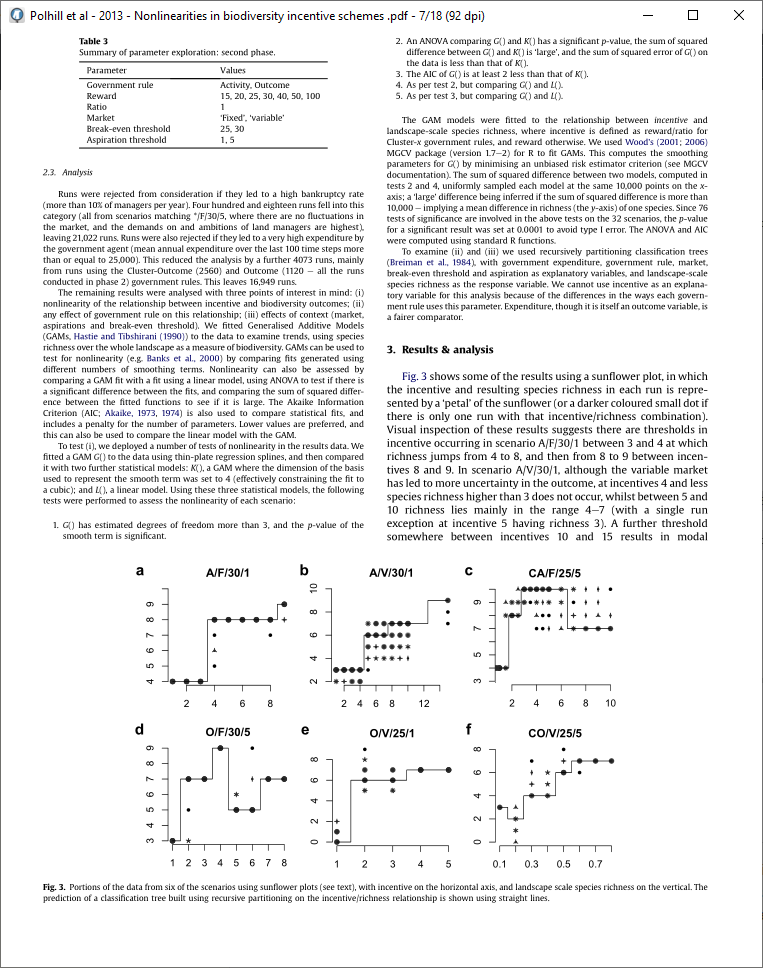
\includegraphics[height=3.5cm]{img/page3.png}};
            \node (img2) at (img1.north east) [yshift=1cm]{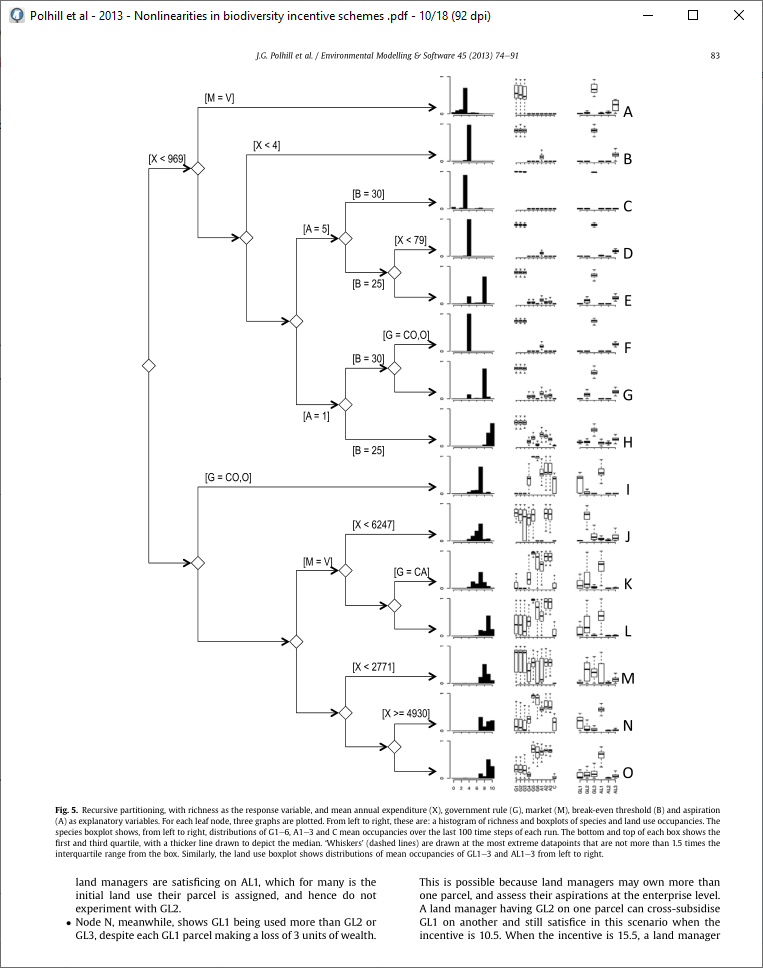
\includegraphics[height=3.5cm]{img/page2.png}};
            \node (img3) at (img2.south east) [yshift=1cm]{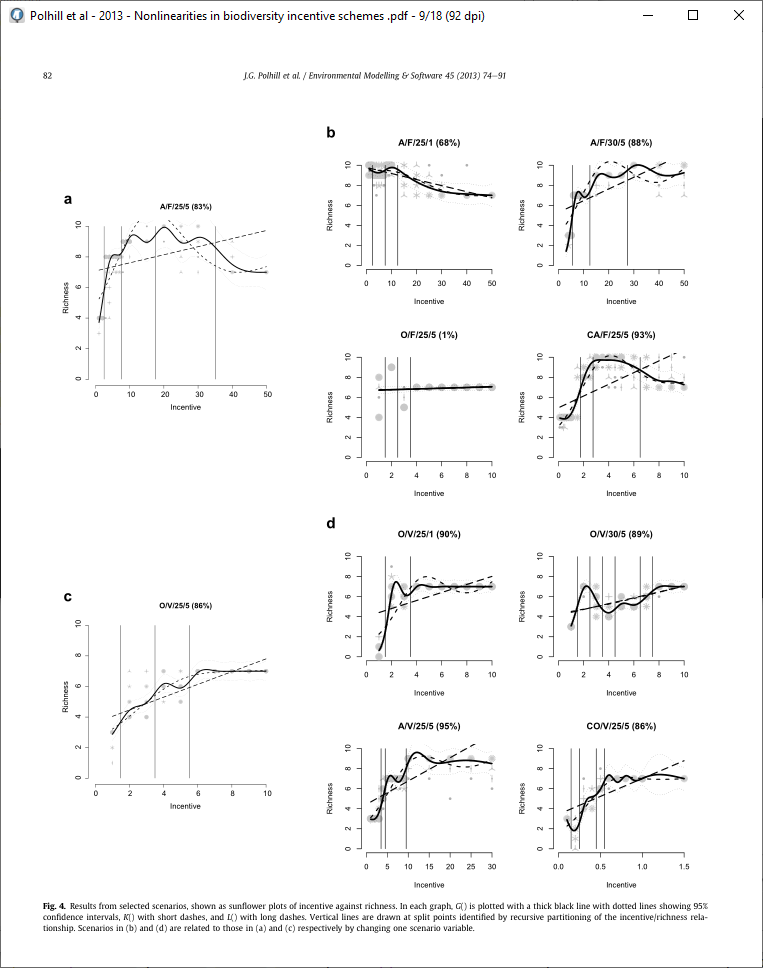
\includegraphics[height=3.5cm]{img/page1.png}};
        \end{tikzpicture}
    \end{center}
\end{frame}

\begin{frame}
    \frametitle{The standard approach}
    \huge
    \begin{itemize}
        \item Scripts 
        \item Storage archives
        \item Diaries
    \end{itemize}
\end{frame}

\begin{frame}
    \frametitle{How we did it}
    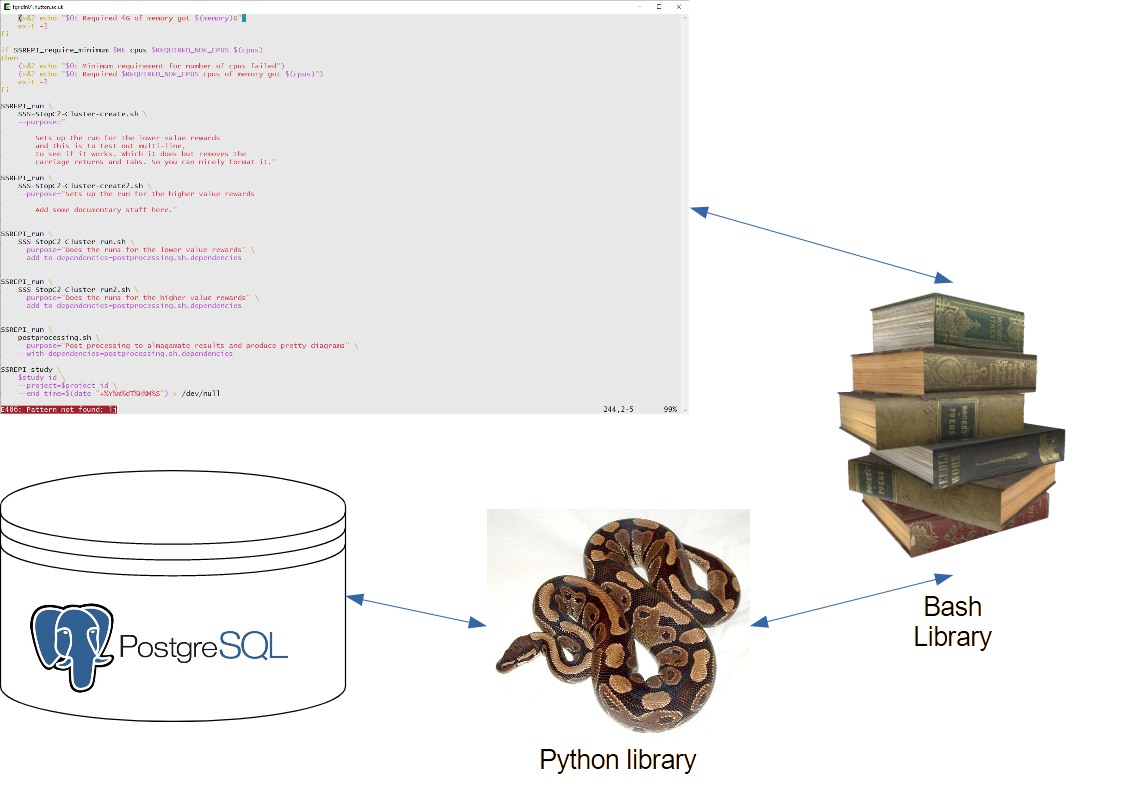
\includegraphics[width=\columnwidth]{img/how.png}
\end{frame}

\begin{frame}
    \center
    \frametitle{The database}

    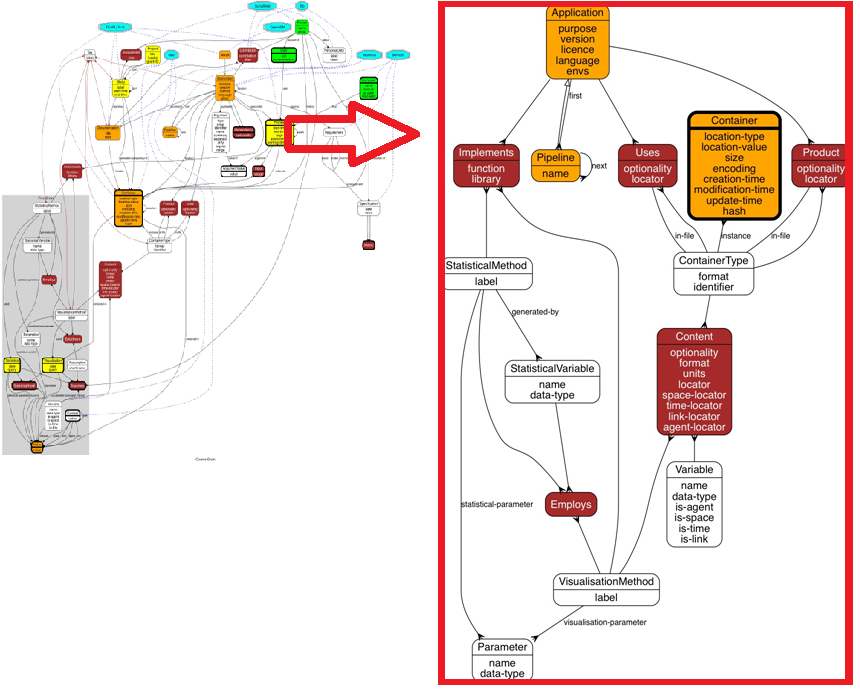
\includegraphics[width=.75\textwidth]{img/schema.png} 

    \large
    \textbf{S}ocial \textbf{S}imultion \textbf{RE}plication \textbf{I}nterface
\end{frame}

\begin{frame}
    \frametitle{The scope}
    \begin{itemize} 
        \item \textbf{Analysis} - fine grain provenance pertaining to statistical and visualisation outputs.
        \item \textbf{Finegrain} - a provenance diagram down to the level of variables.  
        \item \textbf{Folksonomy} - a diagram showing annotations against the database, produced and categorised at the discretion of the user doing the annotation 
        \item \textbf{Project} - management metadata. Largest granularity of metadata supported 
        \item \textbf{Provenance} - provenance diagram at the level of file and parameter 
        \item \textbf{Services} - service provided and requirement description 
        \item \textbf{Workflow} - the actual workflow
    \end{itemize}
\end{frame}

\begin{frame}

    \frametitle{What was needed}
    \tiny
    \begin{table}
        \begin{tabular}{|l|p{1cm}|p{4.8cm}|} 
            \hline 
            Primitive & Type & Purpose \\
            \hline 
            {\color{blue} \ttvar{SSREPI_require_minimum}} & M & Lower bound on software hardware required \\ 
            {\color{blue} \ttvar{SSREPI_require_exact}} & M & Exact bound on software hardware required \\ 
            {\color{blue} \ttvar{SSREPI_application}} & P \& M & specifies some executable \\ 
            {\color{blue} \ttvar{SSREPI_me}} & P \& M & Determines executable or reference to executable being run. \\ 
            {\color{blue} \ttvar{SSREPI_argument}} & P & An argument type to an executable \\ 
            {\color{blue} \ttvar{SSREPI_output}} & P & An output type from an executable \\ 
            {\color{blue} \ttvar{SSREPI_input}} & P & An input type for an executable \\ 
            {\color{blue} \ttvar{SSREPI_person}} & M & Provide metadata for a particular actor within this system \\ 
            {\color{blue} \ttvar{SSREPI_project}} & M & Specifies a project which contains all studies \\
            {\color{blue} \ttvar{SSREPI_study}} & M & A set of experiments makes up a single study \\
            {\color{blue} \ttvar{SSREPI_set}} & M & Sets the default licence and other metadata \\
            {\color{blue} \ttvar{SSREPI_involvement}} & M & Links personnel to a study \\
            {\color{blue} \ttvar{SSREPI_paper}} & M & A paper associated with this study \\
            {\color{blue} \ttvar{SSREPI_make_tag}} & M & Used for building a folksonomy \\
            {\color{blue} \ttvar{SSREPI_tag}} & M & Used to tag any entity with a folksonomy tag \\
            {\color{blue} \ttvar{SSREPI_contributor}} & M & A  person with some kind of relation to an executable or script. \\
            {\color{blue} \ttvar{SSREPI_statistical_method}} & M & Record a statistical method \\
            {\color{blue} \ttvar{SSREPI_visualisation}} & M & Record a method to create an image to depict one or more values. \\
            {\color{blue} \ttvar{SSREPI_statistics}} & M & Record activities that populate the values of statistical variables. \\
            {\color{blue} \ttvar{SSREPI_visualisation_method}} & M & Methods for generating visualisations.  \\
            {\color{blue} \ttvar{SSREPI_implements}} & M & Links a statistical or visualisation method to an application \\
            {\color{blue} \ttvar{SSREPI_parameter}} & M & Record the name taken by a statistical or visualisation method. \\
            {\color{blue} \ttvar{SSREPI_statistical_variable}} & M &  A name for (one of) the result(s) of a statistical method. \\
            {\color{blue} \ttvar{SSREPI_visualisation_variable}} & P \& M & Declares a named variable of interest \\
            {\color{blue} \ttvar{SSREPI_variable}} & M & Names a variable of interest \\
            {\color{blue} \ttvar{SSREPI_statistical_variable_value}} & P \& M & Sets an actual value for a named statistical variable \\
            {\color{blue} \ttvar{SSREPI_value}} & P & Sets a value.         \\
            {\color{blue} \ttvar{SSREPI_content}} & M & Links a kind of output/input/argument to a variable  \\
            {\color{blue} \ttvar{SSREPI_person_makes_assumption}} & M & Links a person to an assumption \\
		 \hline 
        \end{tabular} 
    \end{table}
\end{frame}

\begin{frame}
    \frametitle{What was needed? (cont.)}
    We encoded the previous actions in Python and then then called these from Bash
    \begin{itemize}
        \item {\color{OliveGreen} \ttvar{create_database.py}} - creates a database idempotently.
        \item {\color{OliveGreen} \ttvar{exists.py}} - checks if a particular row in a table exists.
        \item {\color{OliveGreen} \ttvar{get_value.py}} - gets any specified single value from a table given the primary key.
        \item {\color{OliveGreen} \ttvar{get_values.py}}  - gets one or more rows given the search values.
        \item {\color{OliveGreen}\ttvar{next_study.py}} - gets the next available and unique study number. 
        \item {\color{OliveGreen} \ttvar{update.py}} - idempotently updates a particular row in a table.  
    \end{itemize}

\end{frame}


\begin{frame}
    
\includegraphics[width=\textwidth]{img/workflow.png}
\end{frame}

\begin{frame}
    \frametitle{Some provenance!!!}
    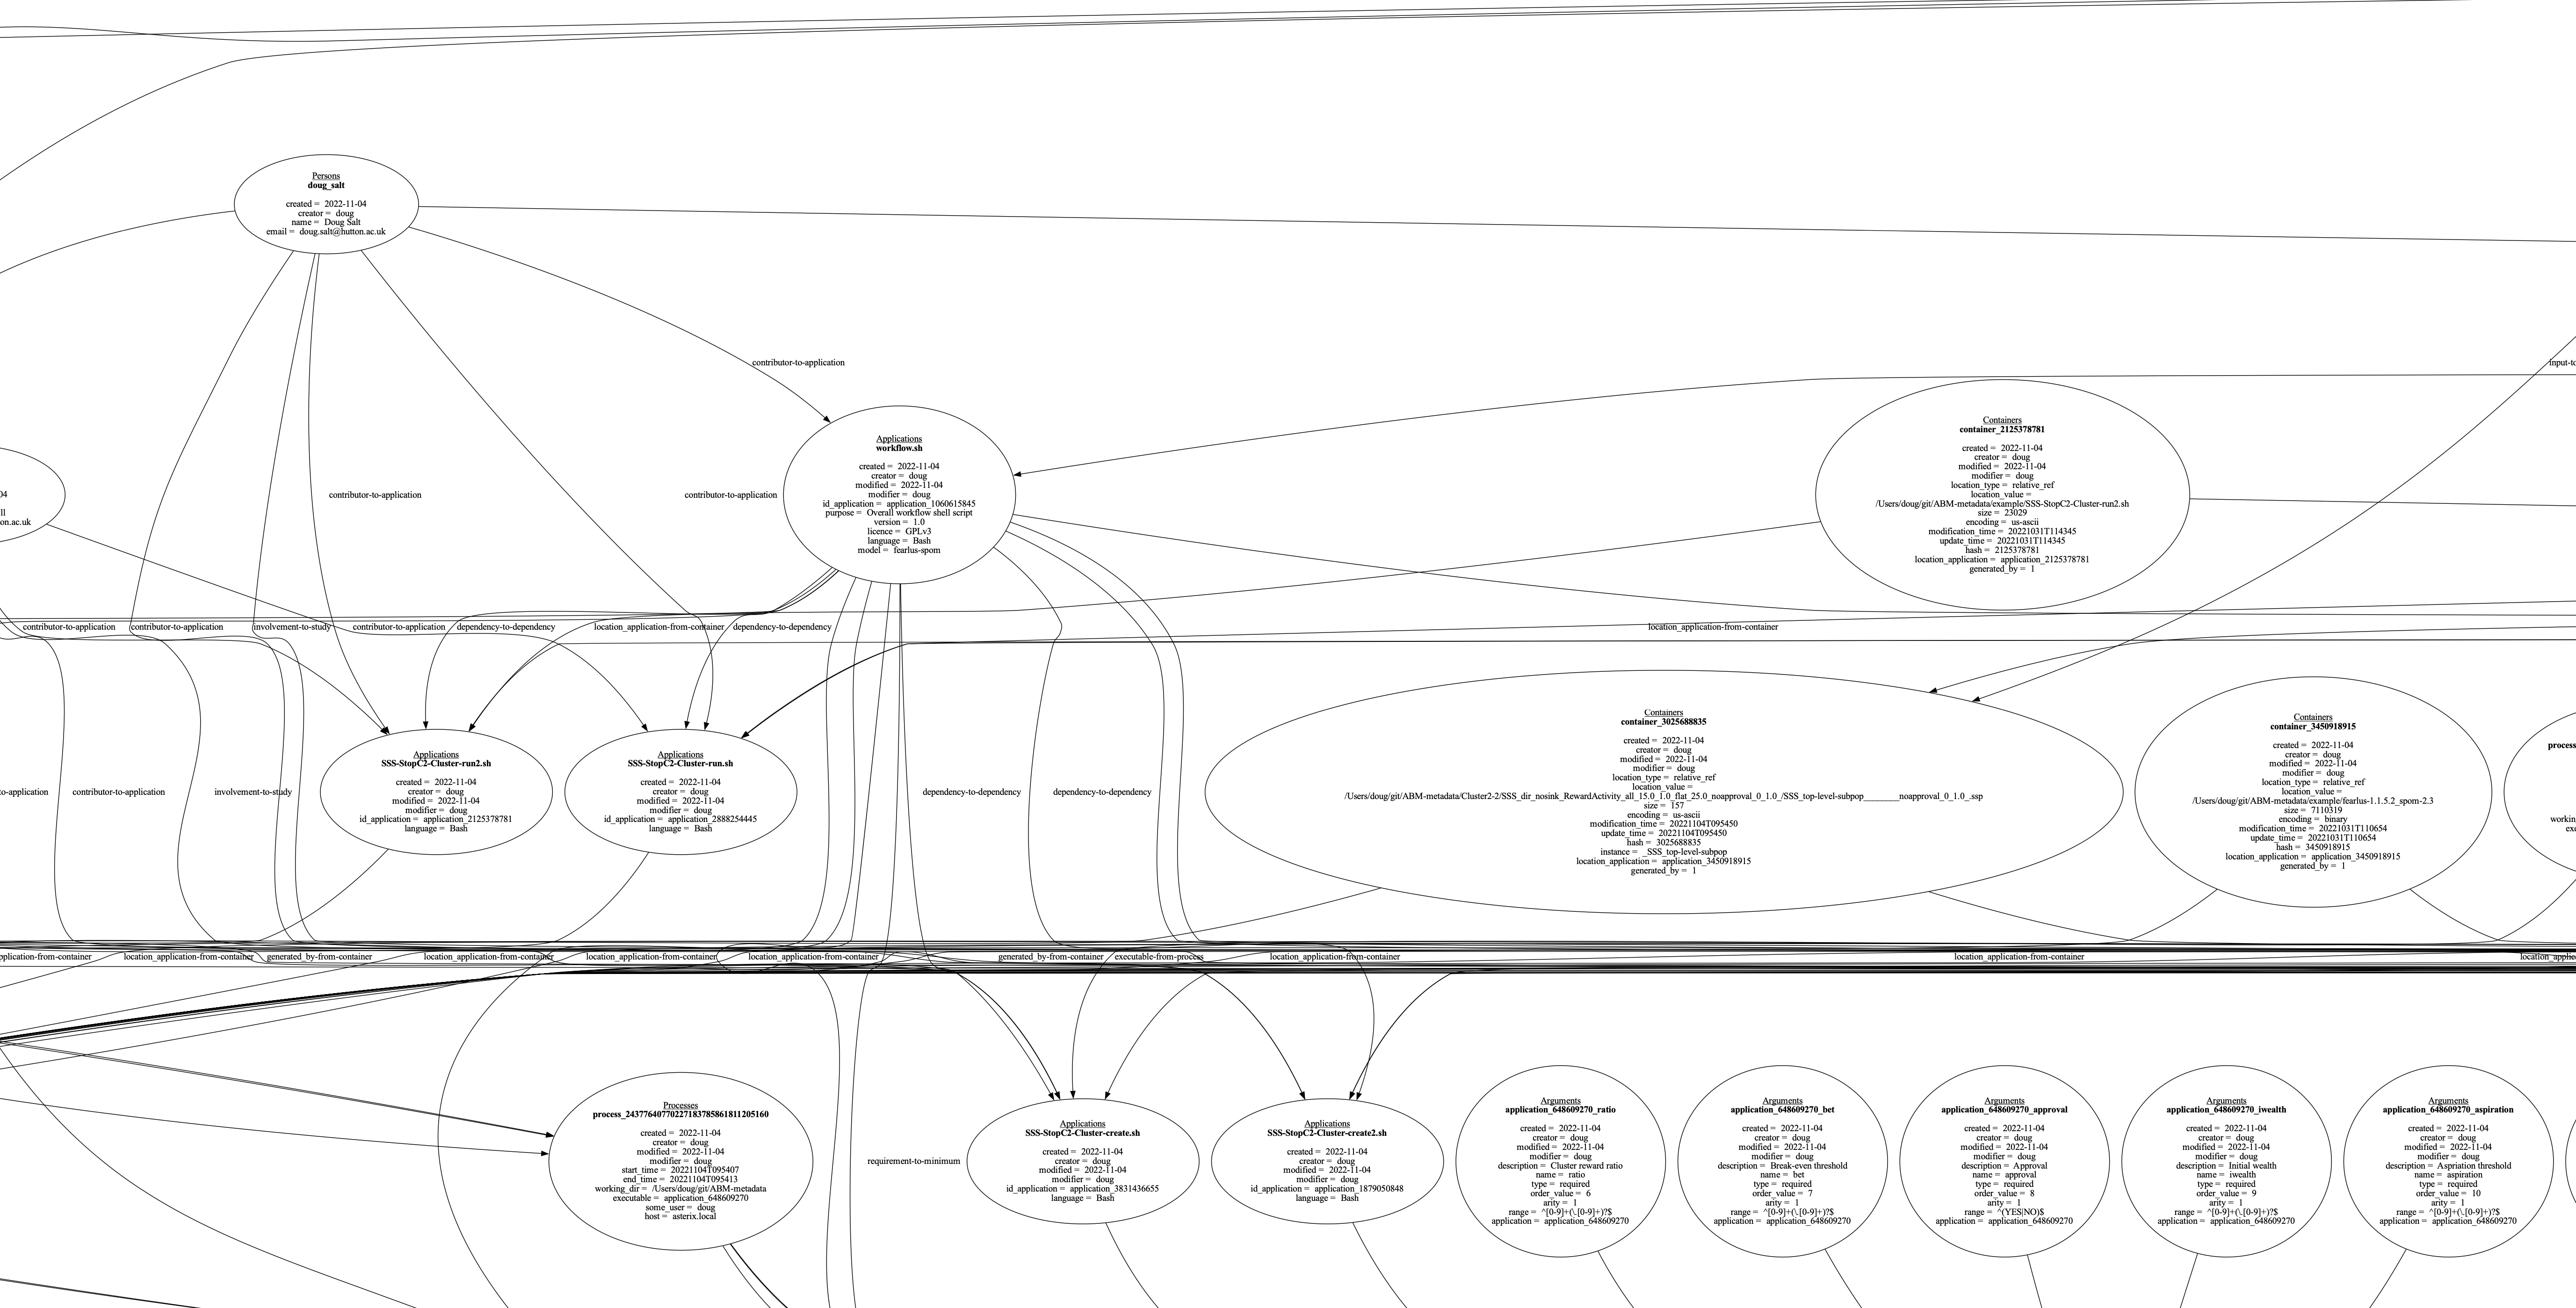
\includegraphics[width=\textwidth]{img/subsection-of-provenance.png}
\end{frame}

\begin{frame}
    \frametitle{So what?}

    It now takes me the following lines of code to reproduce an experiment

    \scriptsize

    \begin{enumerate}
        \item Create new directory
        \item Enter new directory
        \item {\color{blue}\texttt{mkdir bin}}
        \item {\color{blue}\texttt{cp /mnt/storage/doug/git/ABM-metadata/example/*.sh bin}}
        \item {\color{blue}\texttt{cp /mnt/storage/doug/git/ABM-metadata/example/*.pl bin}}
        \item {\color{blue}\texttt{cp /mnt/storage/doug/git/ABM-metadata/example/*.R bin}}
        \item {\color{blue}\texttt{ln -s /mnt/storage/doug/git/ABM-metadata/cfg}}
        \item {\color{blue}\texttt{ln -s /mnt/storage/doug/git/ABM-metadata/lib}}
        \item {\color{blue}\texttt{ln -s /mnt/storage/doug/git/ABM-metadata/doc}}
        \item Amend {\color{blue}\texttt{bin/path.sh}} to {\color{blue}\texttt{bin/path.}}\textit{directory\_name}{\color{blue}\texttt{.sh}}
        \item source {\color{blue}\texttt{bin/path.}}\textit{directory\_name}{\color{blue}\texttt{.sh}}
        \item {\color{blue}\texttt{psql}}
        \item {\color{blue}\texttt{create database third}}
        \item {\color{blue}\texttt{\textbackslash{q}}}
        \item profit!
    \end{enumerate}

\end{frame}

\begin{frame}
    \frametitle{But so what?}
    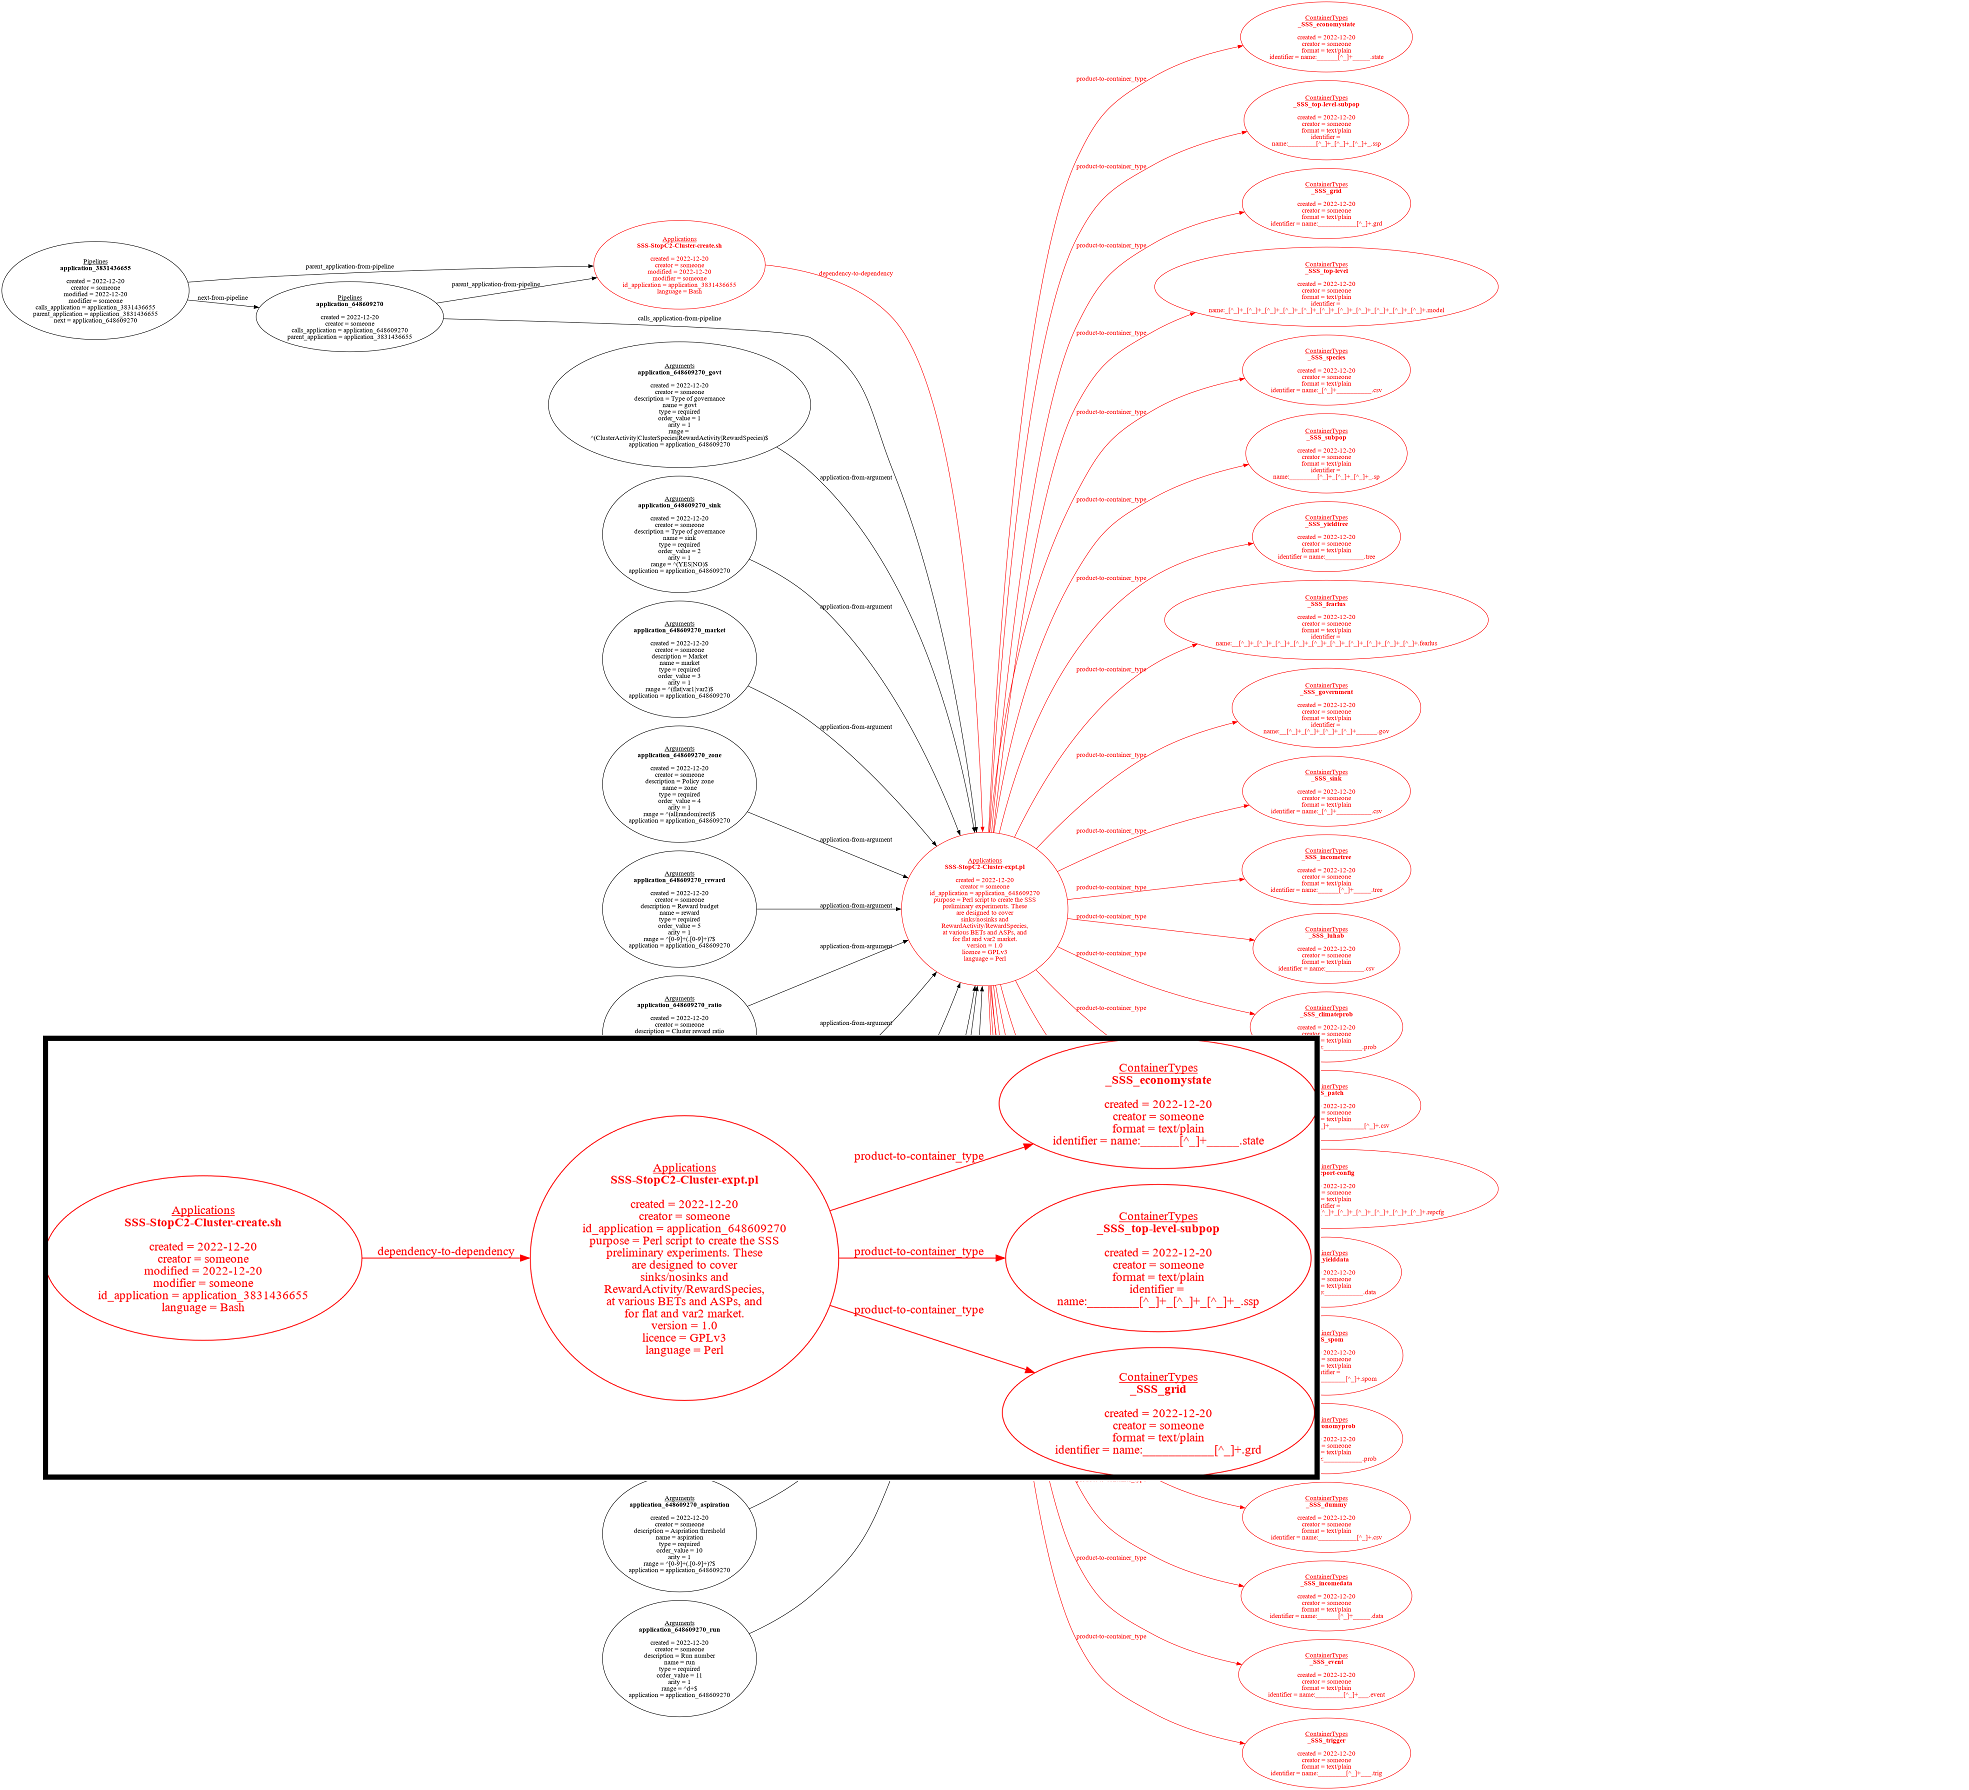
\includegraphics[width=.8\textwidth]{img/broken-application.png}
\end{frame}

\begin{frame}
    \frametitle{Finally a use?}
    \includegraphics[width=\textwidth]{img/high-lit-provenance-trace.pdf}
\end{frame}

\begin{frame}
    \huge
    \center
    \huge
    What else?
    \note{
        1. We are thinking about running AI to look for patterns, if we have a sufficient number of provenace graphs
        2. Modularising and incorporating it into tools so this is automatically generated
        3. Better visualisation
        }
\end{frame}

\begin{frame}[plain]
    Thank you very much
    \finalpage
\end{frame}

\end{document}
